\documentclass[11pt]{article}
\topmargin       -5.0mm
\headheight       0.0mm
\headsep          0.0mm
\oddsidemargin    0.0mm
\evensidemargin   0.0mm
\textheight       210mm
\textwidth        175mm

\usepackage{amsmath,amsfonts,amsthm,amssymb}
\usepackage{latexsym,mathrsfs}
\usepackage{graphicx}
\usepackage{enumerate}
\usepackage{latexsym}
\usepackage{color}
\usepackage{pstricks}
\usepackage{overpic}
\usepackage[ruled,vlined,algosection,linesnumbered]{algorithm2e}
\usepackage{subfigure}
%\usepackage{hyperref}
\usepackage{url}
\usepackage{multirow}

\newtheorem{proposition}{Proposition}[section]
\newtheorem{theorem}{Theorem}[section]
%\newtheorem{algorithm}{Algorithm}[section]
\newtheorem{lemma}{Lemma}[section]
\newtheorem{definition}{Definition}[section]
\newtheorem{corollary}{Corollary}[section]
\newtheorem{remark}{{\sc Remark}}[section]
\newtheorem{example}{Example}[section]

%\numberwithin{algorithm}{section}
\numberwithin{equation}{section}
\numberwithin{figure}{section}
\numberwithin{table}{section}

%%%%%%%%%%%%%%%%%%%%%%%%%%%%%%%%%%%%%%%%%%%%%%%%%%%%%%%%%%%%%%%%%%%%%%%%%%%%%%%%

\begin{document}

\title{Numerical Studies on PSVD Algorithms}

\author{Zheng Wang}

\maketitle

We tested the following PSVD solvers on matrices from LSI and PCA applications, and compare their efficiency and accuracy.

\begin{enumerate}
\item Randomized Block Power method (rsvd\_power): $q = k$, $p = 2$;
\item Randomized Block Krylov method (rsvd\_krylov): $q = 2$, $p = 2$;
\item PROPACK;
\item svds (MATLAB).
\item LMSVD;
\item Block Chebyshev-Davidson method (bchdav\_svd);
\end{enumerate}

% Settings of Computation Environment
All the implementations are in MATLAB 7.8.0 (64-bit), and all experiments are run on the SMUHPC high-memory node with $8$ cores and $144$GB RAM. The compared quantities include \begin{enumerate}
\item CPU time in seconds;
\item relative low-rank approximation error in F-norm
\begin{equation}
err\_mat = \frac{\|\mathbf{A} - \mathbf{U}_k\mathbf{\Sigma}_k\mathbf{V}_k^\mathrm{T}\|_F}{\|\mathbf{A}\|_F};
\end{equation}
\item relative error of each computed singular triplet in 2-norm
\begin{equation}
err\_vec = \frac{\|\mathbf{A}\mathbf{v}_i-\sigma_i\mathbf{u}_i\|_2}{\|\mathbf{A}\|_2}.
\end{equation}
\end{enumerate}

\subsection{Comparison with varying number of computed singular triplets}
\begin{itemize}
\item Experiment on the News20 matrix:\\ 
In bchdav\_svd, $polym = 6$, $blk = 50$, $vimax = 250$. Convergence tolerance ($tol$) is $10^{-8}$ for all algorithms. We gradually increase the number of computed singular triplets ($k$) from $400$ to $2000$ with a stride length $400$. Fig.(\ref{news20_varyk}) shows that our PSVD solver is the fastest with accurate results.

% news20_varyk
\begin{figure}
\centering
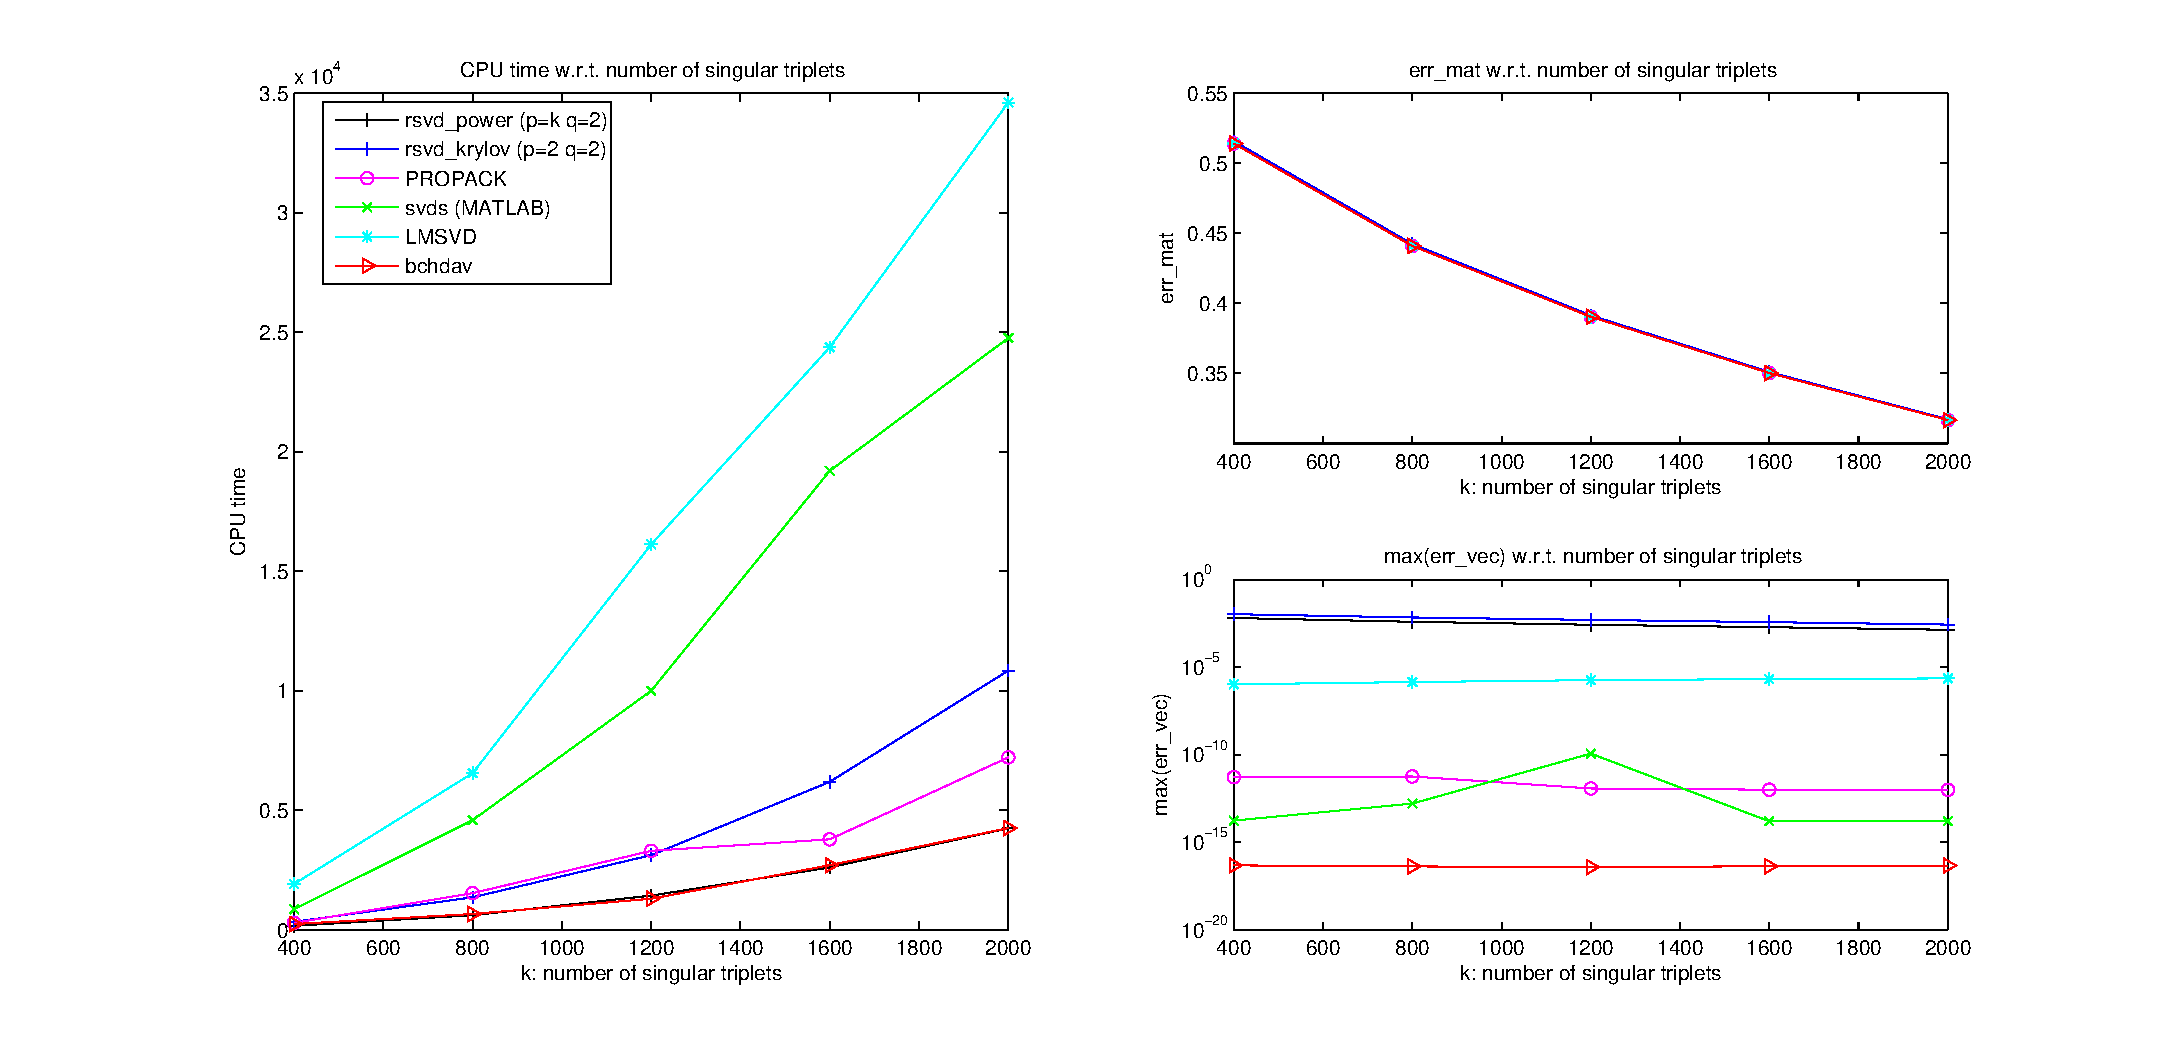
\includegraphics[scale=0.5]{news20_varyk.eps}
\caption{Comparison of CPU time, err\_mat and max(err\_vec) with varying number of computed singular triplets on sparse matrix News20 ($53,975\times11,269$).
}
\label{news20_varyk}
\end{figure}


\end{itemize}
\subsection{Comparison with varying matrix dimension}


\bibliographystyle{plain}
\bibliography{PSVD_bib}


\end{document}
